% Created 2018-02-13 Tue 21:03
\documentclass{article}
\usepackage[mathletters]{ucs}
\usepackage[utf8x]{inputenc}
\usepackage[T1]{fontenc}
\usepackage{fixltx2e}
\usepackage{graphicx}
\usepackage{longtable}
\usepackage{float}
\usepackage{wrapfig}
\usepackage{rotating}
\usepackage[normalem]{ulem}
\usepackage{amsmath}
\usepackage{textcomp}
\usepackage{marvosym}
\usepackage{wasysym}
\usepackage{amssymb}
\usepackage{hyperref}
\tolerance=1000
\author{loli}
\date{\today}
\title{Notebook2}
\hypersetup{
  pdfkeywords={},
  pdfsubject={},
  pdfcreator={Emacs 25.3.1 (Org mode 8.2.10)}}
\begin{document}

\maketitle
\tableofcontents

\section{Edge Detecotr}
\label{sec-1}
\begin{enumerate}
\item Sobel
\label{sec-1-1}
\begin{enumerate}
\item Describing Sobel
\label{sec-1-1-1}
\begin{itemize}
\item This filter works rather similar to linear blur filter from
notebook1, as you are just convoluting a filter over an image.
\item I actually stated what the matrix was for the Sobel filter in
Notebook1, but I shall restate it here and go into why this matrix
makes sense for an edge detector.
\item let S$_{\text{y}}$ =
\begin{pmatrix}
  -1 & -2 & -1\\
  0  & 0  &  0\\
  +1 & +2 & +1
\end{pmatrix}
and let S_x =
\begin{pmatrix}
  -1 & 0 & +1\\
  -2  & 0  & +2\\
  -1 & 0 & +1
\end{pmatrix}
\begin{itemize}
\item Lets consider any pixel at (k,l) with the S$_{\text{y}}$ and S$_{\text{x}}$ filter.
\begin{itemize}
\item the S$_{\text{y}}$ filter will remove the contribution of the pixels on the
same row as the (k,l) pixel, and S$_{\text{x}}$ will do the same to the
vertical pixels as S$_{\text{y}}$
\item Now the interesting part are on the top row of S$_{\text{y}}$ (left column
of S$_{\text{x}}$) and bottom row of S$_{\text{y}}$ (right column of S$_{\text{x}}$). as if you look
at these two, if the color is the same in the neighborhood of
(k,l) then the value should be 0, as the top will cancel out the
bottom (or in the S$_{\text{x}}$ case the left would cancel out the right)
\item This would only leave pixels in which there is a difference
between the top and bottom for S$_{\text{y}}$ and a difference between the
left and right for S$_{\text{x}}$
\end{itemize}
\end{itemize}
\end{itemize}
\item Implementing Sobel
\label{sec-1-1-2}
\begin{itemize}
\item This implementation actually fell out of the discussion session, as
they suggested (since my solution was so general) that I change my
Gaussian kernel into the Sobel one, below is how I ended up defining
the kernel.
\begin{verbatim}
sobelEdgeX :: Num a ⇒ Stencil DIM2 a
sobelEdgeY :: Num a ⇒ Stencil DIM2 a
sobelEdgeX = [stencil2| -1 0 1
                        -2 0 2
                        -1 0 1|]

sobelEdgeY = [stencil2| -1 -2 -1
                         0  0  0
                         1  2  1|]
\end{verbatim}

\item Now that we have the kernel up, lets run them and compose them over the
image (the GHC fuses these two kernel passthroughs into 1).
\begin{verbatim}
sobelX :: (Source r b, Num b) ⇒ Array r DIM2 b → Array PC5 DIM2 b
sobelY :: (Source r b, Num b) ⇒ Array r DIM2 b → Array PC5 DIM2 b
sobelX = mapStencil2 BoundClamp sobelEdgeX
sobelY = mapStencil2 BoundClamp sobelEdgeY


sobel :: (Source r b, Num b) ⇒ Array r DIM2 b → Array D DIM2 b
sobel = R.delay . sobelX . sobelY
\end{verbatim}

\item I rather like running these on colors, even though for edge
detection it doesn't matter, so I ended up generalizing my code for
blurCol (which allows me to blur colored images) so that I can
pass it a kernel to filter the image with.
\begin{verbatim}
with2d f = flip reshape . g . fromList . fmap f . slices <*> R.extent
  where g (RGBA a b c d) = interleave4 a b c d
        g (RGB a b c)    = interleave3 a b c
        g (Grey a)       = a

edgeCol :: (Fractional e, Source r e) ⇒ Array r DIM3 e → Array D DIM3 e
edgeCol = with2d sobel
\end{verbatim}
\begin{itemize}
\item here with2d's logic is already kind of explained with the
\texttt{blurCol} logic in notebook1, basically it just makes 2d slices of
the RGBA bands of an image and applies our filter f (this case sobel).
\begin{itemize}
\item for more detail see notebook1
\end{itemize}
\end{itemize}
\item With all this being done we can actually use sobel and see what
images we get (note I do filter pixels later, but we'll get there).
\begin{itemize}
\item I ended up trying it on two images in the current state.
\item The top left image is the same image used in part1.
\item if you were to look at the full image.
"Color-save-proper-colors.png", you'll notice there is a lot of
noise in this image so the image below won't be surprising.
\item The image on the top right is labeled "Blur-into-Sobo-color.png", as I
ran my Gaussian blur before the Sobel edge detector.
\item Even though it looks rather cool, it really doesn't give much
useful information (I can see some edges in there!).
\begin{figure}
  \centering
  \begin{subfigure}
    \centering
    \includegraphics[width=0.4\textwidth]{../data/Color-test.png}
  \end{subfigure}%
  \begin{subfigure}
    \centering
    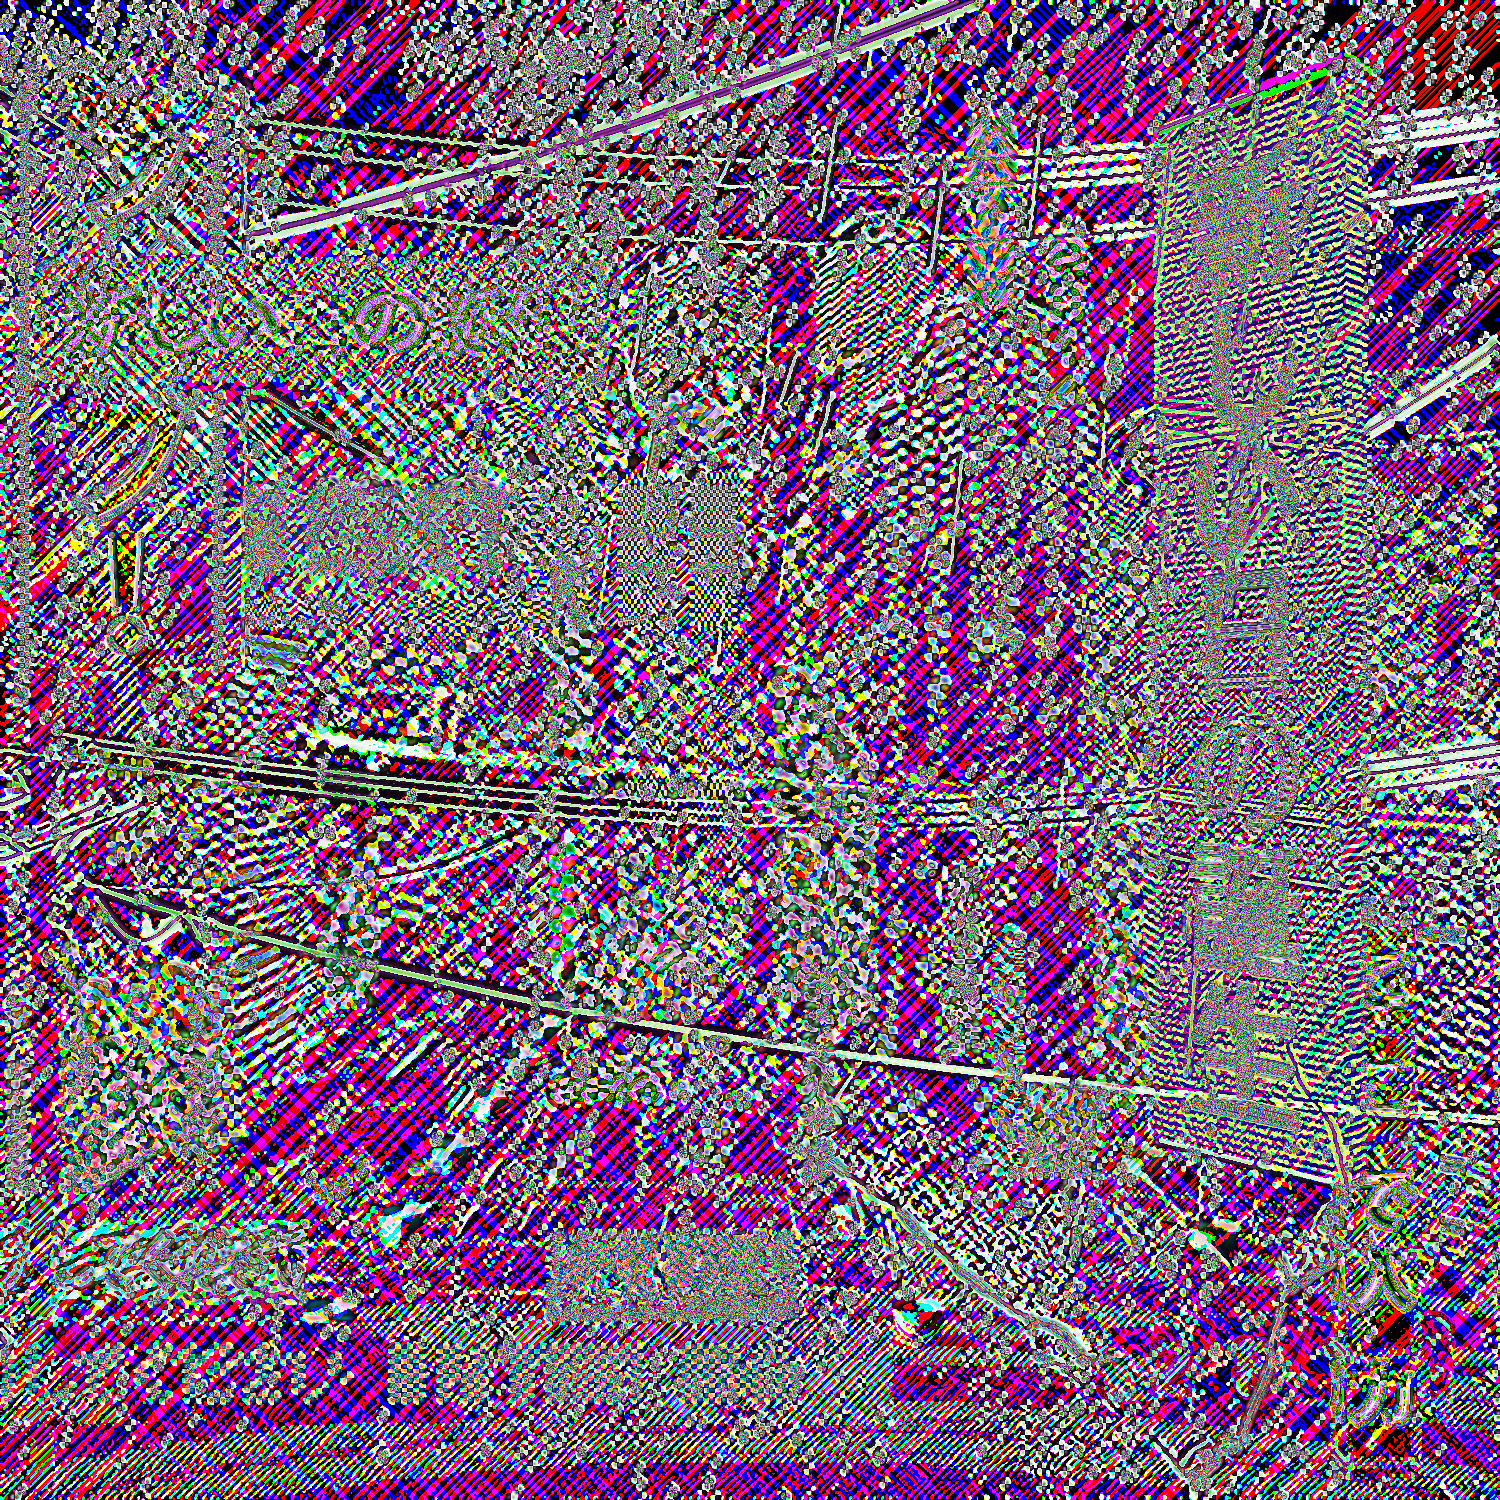
\includegraphics[width=0.4\textwidth]{../data/Blur-into-Sobo-color.png}
  \end{subfigure}
\end{figure}
\item Another image I ran this on was "Colors-wires.png" which can be seen
on the bottom left.
\begin{figure}
  \centering
  \begin{subfigure}
    \centering
    \includegraphics[width=0.4\textwidth]{../data/Color-wires-test.png}
  \end{subfigure}%
  \begin{subfigure}
    \centering
    \includegraphics[width=0.4\textwidth]{../data/Color-wires-blur-then-sobel.png}
  \end{subfigure}
\end{figure}
\item The right shows the output, which does look like edge detection does
take place on a not so noisy image.
\end{itemize}
\item Motivated by the lack of good edges in the noisy image, I decided to
remove all pixels below a certain value as seen below.
\begin{verbatim}
-- type signatures simplified for pdf
filterPixelsS :: Array r DIM3 b → b → Array D DIM3 b
filterPixelsS arr min = R.traverse arr id (passThresh min averaged)
  where
    (Z :. _ :. _ :. k) = R.extent arr
    averaged           = R.sumS $ R.map (/ fromIntegral k) arr

filterPixelsP :: Array r DIM3 b → b → m (Array D DIM3 b)
filterPixelsP arr min = (R.traverse arr id . passThresh min) <$> averaged
  where
    (Z :. _ :. _ :. k) = R.extent arr
    averaged           = R.sumP $ R.map (/ fromIntegral k) arr

-- helper for filterPixelP and S
passThresh min avg f sh@(Z :. i :. j :. _) | avg ! ix2 i j >= min = f sh
                                           | otherwise            = 0
\end{verbatim}
\begin{itemize}
\item Here we really traverse the old image and compare it with the
average value at that point, and if it's below our threshold we just
say it's 0. Also note that there is \texttt{filterPixelsS} and
\texttt{filterpixelsP} because I noticed that all my cores weren't being
used when the S version was being run
\begin{itemize}
\item I would show "colores-blur-then-sobel-100",
"colores-blur-then-sobel-210", and
"Color-wires-blur-then-sobel-100-min.png", but sadly they don't
show up too well on the pdf, but it was rather interesting to
see what details went away when the min value was changed.
\end{itemize}
\end{itemize}
\end{itemize}
\end{enumerate}
\item Canny
\label{sec-1-2}
\begin{enumerate}
\item Describing Canny
\label{sec-1-2-1}
\begin{itemize}
\item The canny edge detector can be broken into a few discrete steps that
I've sourced from Wikipedia
\begin{enumerate}
\item Find the intensity gradients of the image
\item Apply non-maximum suppression to get rid of spurious response to
edge detection
\item Apply double threshold to determine potential edges
\item Finalize the detection of edge by suppressing all other edges
that are weak and not connected to strong edges
\end{enumerate}
\end{itemize}
\item Implementing Canny
\label{sec-1-2-2}
\begin{itemize}
\item There is a package for Haskell, called \texttt{friday} that has a cannyEdge
detector built in, so I ended up using that.
\begin{verbatim}
cannyEdge :: Int -> Int32 -> Int32 -> Image PixelRGB8 -> I.Grey
cannyEdge radS min up = canny radS min up . toGrey . toFridayRGB
\end{verbatim}
\item I ended up using my Gaussian blur to preprocess the image, as the
library does not do that for me (edge detectors are quite sensitive to
noise, and blurring helps with that).
\item the Libraries version only works for Grey images sadly, however it
did a better job than the Sobel detector at edge detector on the 2
images I compared it with.
\begin{figure}
  \centering
  \begin{subfigure}
    \centering
    \includegraphics[width=0.45\textwidth]{../data/grey-wires-canny-5-120-300.png}
  \end{subfigure}%
  \begin{subfigure}
    \centering
    \includegraphics[width=0.45\textwidth]{../data/grey-canny-5-120-300.png}
  \end{subfigure}

  \begin{subfigure}
    \centering
    \includegraphics[width=0.45\textwidth]{../data/grey-canny-3-120-300.png}
  \end{subfigure}
\end{figure}
\begin{itemize}
\item The top two were run with radius 5, while the bottom one was run
with radius 3.
\item For a really noise image at 1500x1500 size, that a smaller radius
is preferable.
\begin{itemize}
\item Further tests with a 3872x2592 image of trees also confirms this
as at radius two, the edge detection was rather good, but at
radius 5 I would need to filter out a lot more (this could just
be caused with brighter values sneaking its way in!).
\end{itemize}
\end{itemize}
\end{itemize}
\end{enumerate}
\end{enumerate}
\section{General Notes on performance}
\label{sec-2}
\begin{itemize}
\item In general I'm rather proud of the performance. The Sobel filter
with all colors running take less than 40 seconds to run on a
1500x1500 image.
\item Also the code provided hammers all 8 of my cores without stopping
(except when I run \texttt{filterPixelS}, but I don't ever run this)
\begin{itemize}
\item The best part about this, is the only word I speak of parallel
code is \texttt{filterPixelP} and the 2 \texttt{computeUnboxedP} in the main
function.
\end{itemize}
\item The speed of this allows me to quickly test out what happens if I
say only use the SobelX but not SobelY
\end{itemize}
% Emacs 25.3.1 (Org mode 8.2.10)
\end{document}